\section{Results}

\subsection{Number of planets}
To investigate how the number of planets changes during a 5000 years evolution of a solar system and how it varies with the parameter $N$(initial number of bodies). We varied $N$ from $100$ to $1000$ with step size $100$(thus 10 different $N$'s). For each $N$, we ran 5 simulations measured the average number of planets after every 10 years. The following results are obtained:\\ 
\begin{figure}[H]
\centering
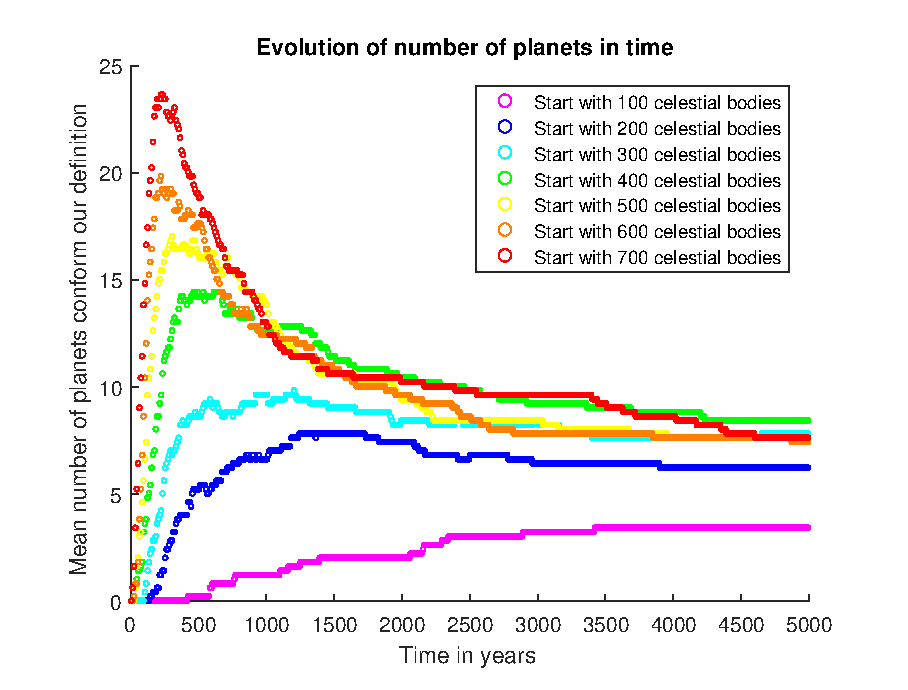
\includegraphics[scale=0.8]{AantPlaneten.eps}
\caption{Average number of planets during 5000 years of evolution, measured after each 10 years}
    \label{fig:AantPlaneten}
\end{figure}
As is shown in Figure \ref{fig:AantPlaneten}, planets are quickly formed in the early stadium of the evolution, and the more bodies there are, the more planets are formed in this stadium. This is logical, since the system is very dynamic in the early stadium due to the huge amount of bodies that gives rise to many collisions. After this early stadium, the small planets accrete further and become bigger planets, and the system becomes more and more stable until a sort of equilibrium is reached in which the number of planets is constant.\\

Note that although a larger number of bodies at the start would result in a larger number of planets at the early stadium, the number of planets at the end is roughly the same independent of $N$, if $N$ is large enough(in our case around $N=300$). This is quite expected, since a larger $N$ would mainly results in larger planets. And this is confirmed...

